\section{Results}
The model receives a reward ($+1$) every second that trunk lean is less than $30^{\circ}$. Figure \ref{fig:boxplot} shows variation of reward with respect to number of training iterations for $10$, $20$, $30$ and $40$ million. In this figure, red line indicates mean value, horizontal lines maximum and minimum values. Likewise, the reward that model gets with $20$ million is greater than with $10$ million. This is because the model learns to walk better with more training time. However, the reward that model gets with $30$ and $40$ million is less than with $20$ million. This is because model is trying/learning to use both legs instead of just one\footnote{visual material of the training of the two-legged robot in \url{https://www.youtube.com/watch?v=Vt20_SWR2xI&ab_channel=LucaBorgonovi}}.


\begin{figure}
	\centering
	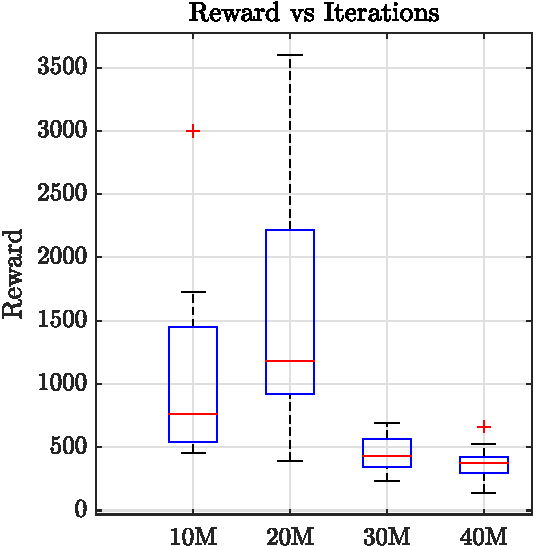
\includegraphics{images/reward_vs_iter.pdf}
	\caption{Performance of trained model to keep the trunk lean below $30^{\circ}$.}
	\label{fig:boxplot}
\end{figure}


The Policy Gradient algorithm was implemented in Python language using the TensorFlow library, which is an open-source library for artificial intelligence and machine learning.

To carry out the simulations, the MuJoCo software was used (Multi-Joint Dynamics with Contact), a simulator for multi-body dynamics with contact. The computational model used to implement the algorithm was a two-dimensional bipedal robot Walker2d-v2, which has 7 joints and two translational movements (horizontal and vertical). During the simulation, the model went through 40 million states to assess how gait evolved as the Policy Gradient algorithm was implemented.

All simulations were carried out on a computer with Intel\textregistered Core\texttrademark i7-8750H 2.20 GHz processor, 8.00 GB of RAM, 128 MB dedicated video card, Windows 10 Home Single Language 64 bits. The Python version XXX and the MuJoCo XXX were the platforms where the simulations took place.
